\documentclass{mpaper}

\usepackage[boxed]{algorithm2e}

\begin{document}

\title{Machine Learning on EEG Signals for Predicting Central Neuropathic Pain in Spinal Cord Injury Patients \newline \large{Masters project dissertation - MSci SEWP 40 credit project}}
\author{Cristian-Liviu Chirion}

\matricnum{2188639C}

\maketitle

\begin{abstract}
Central Neuropathic Pain (CNP) is a condition that can greatly interfere with a patient's life, and often leads to mental health issues and even suicide. It is common in people who have previously suffered Spinal Cord Injury (SCI) and a cure for it is not presently available. Detecting this condition early, before the onset of its symptoms, would provide an opportunity for more efficient treatment and could motivate further research of cures or preventive treatments. In this study, we explore Electroencephalography (EEG) data from SCI patients as a potential means of detecting CNP with the help of machine learning techniques. We experiment with several data processing, feature extraction, and classification methods and discuss the results, while also analyzing the available data. We find several promising results, with our best classifier being able to distinguish between the EEG recordings of patients with pain and those of patients without pain with an accuracy of 96\%. 
\end{abstract}

\section{Introduction}

\subsection{Motivation}

Spinal Cord Injury (SCI) is known for its potential to cause significant harm to the human body, often reducing a patient's mobility by rendering one or more limbs unusable. Another issue that can appear as a result of SCI is the onset of Central Neuropathic Pain (CNP), which currently has no known cure and is frequently strong enough to interfere with the patient's sleep and daily routines, often leading to serious mental health issues {\cite{hulsebosch_mechanisms_2009}}.

There are various treatments available for CNP patients which can reduce the pain to tolerable levels. Antidepressants, for example, have been shown to be beneficial in mitigating neuropathic pain~\cite{finnerup_review_2008}, but they often cause significant side effects such as drowsiness, fatigue, bladder issues, digestive issues, which can further interfere with a patient's life~\cite{finnerup_review_2008,khawam_side_2006}.

Being able to accurately predict whether a patient is likely to develop CNP in advance of the pain actually appearing would offer the opportunity to administer preventive treatments and could motivate new pharmacological studies for developing more efficient pain prevention medication.

\subsection{Prediction of CNP}

Electroencephalography (EEG) is a technique for monitoring and analysing brain activity by placing multiple sensors across a patient's scalp and using them to measure the intensity of electrical activity over time in various parts of the brain. Individual sensors are referred to as 'channels', each channel representing a different location on the scalp~\cite{noauthor_multi-channel_nodate}. There have been various studies that concluded that there are statistically significant differences between the EEG signals of SCI patients without CNP and SCI patients who have developed or are about to develop CNP~\cite{vuckovic_prediction_2018}. This provides an opportunity for researching machine learning techniques to classify SCI patients based on whether they develop pain or not, thus making it possible to predict the onset of CNP.

\subsection{Statement of problem}

The goal of this study was to create one or more machine learning models that can accurately distinguish the SCI patients who have CNP from those who do not, as well as the SCI patients who will later develop CNP from those who will never develop CNP, based on their EEG recordings. We focused on exploring different approaches to data pre-processing and feature extraction, combining methods which have been shown to be efficient in previous EEG studies with techniques that have not previously been used in this field, but are frequently used in machine learning problems.

We report on the methodology and results for each of the experiments we conducted, analyzing the behaviour of the various classification approaches, as well as noting any relevant patterns or features we found in the data as a result of this study. We also discuss the relevance of our results and the contributions of this paper, highlighting any limitations, as well as opportunities for further research.

\section{Background}

\subsection{Opportunity for classification}

EEG as a brain activity monitoring method is most commonly encountered in brain-computer interface (BCI) technologies~\cite{wolpaw_brain-computer_2000}, which have been successfully used in the diagnosis of various medical conditions such as sleep disorders~\cite{min_medical_2009} and epilepsy~\cite{acharya_automated_2013}. Significant research is also being conducted in using BCIs to mitigate the effects of various conditions, such as improving communication for patients with autism or speech disorders, and facilitating daily activities for those with reduced muscle control~\cite{wolpaw_brain-computer_2000}.

For the purpose of this study, we hypothesise that the differences between the EEG signals of patients with pain and patients without pain can allow us to classify the two categories using machine learning techniques. This assumption is justified by previous research where such EEG signals were analyzed and statistically significant differences between the two groups were found~\cite{vuckovic_dynamic_2014,jarjees_causality_2017}, meaning that there could be an opportunity to classify these two groups based on their EEG data.

We reviewed several previous studies involving EEG analysis in order to assess potential methods for data processing, feature extraction and classification. The research provided by Vuckovic et al.~\cite{vuckovic_dynamic_2014} was particularly useful since it was performed on the same data that we used in this project.

\subsection{Data pre-processing and feature extraction}

In most machine learning problems, it is important to apply efficient processing and feature extraction methods in order to make the most of the available data. This is particularly important in our case, since the EEG signal data is in the form of time series of voltage sampled at a high rate (250Hz) across a large number of channels (48-61), meaning that a machine learning model created from the raw data would be high-dimensional, and would be susceptible to the 'curse of dimensionality', which dictates that the required size of a data set to train a model increases exponentially with the number of dimensions. Given this high dimensionality, as well as the fact that our data sets are small, a significant part of this study was dedicated to exploring approaches to reducing the dimensionality of the data and selecting subsets of channels to be used for classification.

Band power transformations based on Fast Fourier Transforms (FFT) are commonly mentioned in literature as a method for processing EEG signals, including the study conducted by Vuckovic et al.~\cite{vuckovic_dynamic_2014}. This approach involves mathematically transforming the signal from the time domain into the frequency domain, and estimating the power spectral density (PSD) over different frequency intervals, commonly referred to as 'bands'. Most of the research in this field has found three frequency bands that contain useful information about EEG activity: theta (4Hz to 8Hz), alpha (8Hz to 13Hz) and beta (13Hz to 30Hz). Although the exact definitions of the bands vary slightly across different studies (e.g. Vuckovic et al.~\cite{vuckovic_dynamic_2014} use a beta band of 16-24 Hz, while other studies include frequencies as low as 12.5 Hz and as high as 30 Hz in this band~\cite{rangaswamy_beta_2002, subasi_neural_2005}), there is a consensus in literature that these three frequency bands are useful for analyzing EEG data~\cite{jarjees_causality_2017,rangaswamy_beta_2002,subasi_neural_2005,vuckovic_prediction_2018,vuckovic_dynamic_2014}.

Klonowski~\cite{klonowski_everything_2009} discusses that, although FFT approaches have been seen to perform well on EEG data, methods involving time series analysis could be more useful in preserving the information from the original signals. A notable example of such a method is Higuchi's fractal dimension, proposed by Higuchi~\cite{higuchi_approach_1988}, which involves applying a mathematical formula which assesses the complexity of the time signal, returning a 'fractal dimension' value between 1 and 2 - where a higher value means a more complex signal. An advantage of this approach is that the entire signal is reduced to a single value, thus the dimensionality is drastically reduced.

Another approach that we chose to include in this study was Principal Component Analysis (PCA), a more generic mathematical approach to dimensionality reduction, which projects the data points onto a smaller, pre-defined number of orthogonal axes or 'components', in such a way that the variance among data points is maximized~\cite{kumar_understanding_2018,wold_principal_1987}. Although this method is not particularly common in previous EEG research, we decided to include it as a standard mathematical procedure which performs the key function we are looking for: reduce the dimensionality while keeping potentially useful features of the data by maintaining a high variance. 

We also decided to explore classification on the raw EEG signals. Although this approach has the previously discussed disadvantage of high dimensionality, there have been studies, such as the one conducted by Kaper et al.~\cite{kaper_bci_2004}, that found raw time-domain signals to produce decent classification results as long as a sensible subset of channels was selected.

We performed extensive comparative evaluations of various combinations of the methods mentioned above.

Regardless of how the data is processed and input into a classifier, an important step in extracting features was to select a subset of channels that maximizes classification accuracy. Since the various channels contain information about activity from different parts of the brain, it is sensible to expect that certain channels will be more useful than others in detecting patients with EEG~\cite{vuckovic_dynamic_2014}. For the purpose of channel selection, we used a sequential process described in more detail in section \ref{procedure}.

\subsection{Classification}

A key decision we took in terms of scoping this project was that we would prioritize experimenting with data processing and feature selection methods rather than trying a large number of classifiers. As a result, we only included two classification methods in this study.

K-Nearest Neighbours (KNN) was chosen mainly because of its simplicity of implementation of evaluation~\cite{harrison_machine_2019}, providing a good option for initial classification attempts. Although it is not likely to outperform more complex classifiers, this method proved to be a useful approach for obtaining initial baseline results for the various data processing methods we experimented with.

Linear Support Vector Machines (SVM) is a classifier that involves representing the training data points in a multi-dimensional vector space and finding a hyperplane that separates the data points from different classes, while maximizing the distance between the hyperplane and the data points closest to it, which are referred to as 'support vectors'~\cite{gandhi_support_2018}. This method has been used successfully in a significant number of EEG classification problems, usually outperforming other classifiers, in part thanks to its ability to classify relatively small data sets~\cite{lotte_review_2007}. Examples of studies on EEG that obtained good results from linear SVM classification include Vuckovic et al.~\cite{vuckovic_prediction_2018}, who obtained a 76\% accuracy, and Kaper et al.~\cite{kaper_bci_2004}, who obtained a 84.5\% accuracy.

\section{Methodology}

\subsection{Methods}

Below we present a summary of the data processing methods applied in the experiments we ran.

\subsubsection{Raw EEG time series}

Raw series of EEG signals from the selected channels were input into the classifiers for each iteration. There was no pre-processing applied to the data. The classifier thus received an input of size [\( number\ of\ channels \times number\ of\ readings \)], which was flattened into a one-dimensional array before being used for training the classifier.

\subsubsection{Band power transformations}
\label{bandpower-method}

The EEG series in each channel was transformed from the time domain into the frequency domain by calculating the power over each of three frequency bands: theta (4Hz to 8Hz), alpha (8Hz to 13Hz) and beta (13Hz to 30Hz). The classifier input therefore had a size of [\( number\ of\ channels \times 3 \)]. The implementation of the band power transformations made use of the Python-based Scipy\footnote{https://www.scipy.org/} library, and involved calculating the power over all frequencies in the frequency spectrum using a Fast Fourier Transform, then performing an integration operation on the three relevant frequency intervals to obtain our three band power values.

\subsubsection{Higuchi's fractal dimensions}

The Higuchi fractal dimension value was calculated for each channel's time series using an open source Python implementation\footnote{https://github.com/inuritdino/HiguchiFractalDimension}. This procedure involves finding the average curve length $L(k)$ over $k$ estimations of the time series curve length, where each curve length $L(k)$ is calculated based on splitting the curve into intervals of size $k$. The process is repeated for multiple, logarithmically increasing values of $k$, with $L(k)$ being calculated for each value of $k$. The fractal dimension $D$ is then computed such that, if the $L(k)$ values are plotted against the $k$ values on a logarithmic scale, the data points fall on a straight line with slope $-D$~\cite{higuchi_approach_1988}.

Since the fractal dimension, and thus the complexity of each time signal, was represented by just one value, the classifier input had a size of [\( number\ of\ channels \times 1 \)].

It should be noted that the fractal dimension was not calculated based on the entire time series. Given that this technique is known to be more accurate and more efficient for shorter time series~\cite{kesic_application_2016}, we only used a half-second interval from t=1.5s to t=2.0s for estimating this value. This time frame was chosen because it was shortly after the initiation cue that instructed patients to imagine movements, thus it was the interval during which we expected the strongest response in the patients' brain activity.

\subsubsection{Principal Component Analysis (PCA) on time series}
\label{pca-method}

A Scikit-Learn implementation of PCA was used to reduce the dimensionality of each time series. This technique involves projecting the initial data points onto a smaller, pre-defined number of new orthogonal axes, in such a way that the variance between different data points remains as high as possible. We used a number of three 'components' or axes for each channel, thus the size of the classifier input for this method was [\( number\ of\ channels \times 3 \)].

\subsubsection{Principal Component Analysis (PCA) on frequency bands}

For this approach, we combined the band power transformation and PCA methods described in sections \ref{bandpower-method} and \ref{pca-method} respectively. Band power transformations were first applied to the time series in order to reduce each channel to three values representing the three power bands. The band power values for the selected channels were concatenated, and the resulting array of size [\( number\ of\ channels \times 3 \)] was transformed using PCA into a set of three components. This means that the classifier input with this method was an array of size 3, regardless of how many input channels were selected.


\subsection{Procedure}
\label{procedure}

The implementation part of the project involved running experiments with each of the following methods:

\begin{itemize}
    \item Raw EEG signals and KNN classifier
    \item Raw EEG signals and SVM classifier
    \item Band power transformed signals and KNN classifier
    \item Band power transformed signals and SVM classifier
    \item Higuchi's fractal dimension and KNN classifier
    \item Higuchi's fractal dimension and SVM classifier
    \item PCA applied to raw EEG, and KNN classifier
    \item PCA applied to band power transformed signals, and KNN classifier
\end{itemize}

For each of the above, the goal was to apply the relevant processing technique to the data, then feed it into a classifier and optimize it in order to maximize its performance, based on the evaluation criteria defined in section \ref{model-eval}. The main variables that we sought to adjust when optimizing were the channels being included in classification, and the classifier hyper-parameters - k value (number of neighbours) for KNN and nu value (minimum proportion of support vectors) for SVM.

The subset of channels to be used for each method were chosen through a 'greedy' approach of training and testing the classifier on each individual channel over multiple iterations, checking which one would increase accuracy the most by being used as classification input. This was done until it was not possible to increase accuracy further by adding more channels. It should be noted that this approach is not guaranteed to find the overall combination of channels that gives the best results. However, since the number of channels was high (61 for the PP/PNP data sets), trying all possible combinations was unrealistic. We therefore chose this 'greedy' procedure as a way to test many combinations of channels and find one which is likely to be better than most others, without taking an excessively long time to compute. A high-level pseudocode of the channel search process is presented in Algorithm \ref{channel-search}.

\begin{algorithm}
    \SetKwInOut{Input}{Input}
    \Input{data - pre-processed EEG series}
    \SetKwInOut{Output}{Output}
    \Output{channels - list of channels to use in classification}
    \BlankLine
    best accuracy = 0\;
    previous accuracy = 0\;
    previous channels = empty list()\;
    
    \While{best accuracy >= previous accuracy}{
    
        previous accuracy = best accuracy\;
        
        \If{best channel exists}{
            previous channels.add(best channel)\;
        }
    
        \For{channel in data.channels}{
            
            // Get the data for the selected channels\;
            d = data.get(previous channels + channel)\;
            accuracy = train and cross validate(d)\;
            
            \If{accuracy > best accuracy}{
                best accuracy = accuracy\;
                best channel = channel\;
            }
        }
    }
    channels = previous channels\;
    
    
    \caption{Channel selection}
    \label{channel-search}
\end{algorithm}

The classification hyper-parameters, including the k value for KNN and the nu value for SVM, were chosen by iterating over many of their possible values, finding the ones that yielded the best results, and subsequently narrowing the range of possible values in order to try to further improve accuracy. For example, finding a good value for the SVM nu parameter, which is a fraction between 0 and 1, involved initially iterating from 0 to 1 with a step size of 0.01. If the best-performing value in this range was found to be 0.6, the experiment was repeated on a narrower interval of 0.59 to 0.61, with a reduced step size of 0.001.

Algorithms \ref{k-search} and \ref{nu-search} present high level pseudocode descriptions of the hyper-parameter tuning process for KNN and SVM respectively.

\begin{algorithm}
    \SetKwInOut{Input}{Input}
    \Input{data - pre-processed EEG series}
    \Input{channels - pre-selected channel subset}
    \SetKwInOut{Output}{Output}
    \Output{k value hyper-parameter}
    \BlankLine
    best accuracy = 0\;

    min k = 1\;
    max k = 150\;
    step = 10\;

    \For{k=min k, k<max k, k+=step}{
            
        // Get the data for the selected channels\;
        d = data.get(channels)\;
        accuracy = knn train cross validate(d, k)\;
        
        \If{accuracy > best accuracy}{
            best accuracy = accuracy\;
            best k = k
        }
    }
    
    min k = max(min k, best k - step)\;
    max k = min(max k, best k + step)\;
    step = 1
    
    \For{k=min k, k<max k, k+=step}{
        
    // Get the data for the selected channels\;
    d = data.get(channels)\;
    accuracy = knn train cross validate(d, k)\;
    
    \If{accuracy > best accuracy}{
        best accuracy = accuracy\;
        best k = k
    }
}
    
    \caption{KNN k value selection}
    \label{k-search}
\end{algorithm}

\begin{algorithm}
    \SetKwInOut{Input}{Input}
    \Input{data - pre-processed EEG series}
    \Input{channels - pre-selected channel subset}
    \SetKwInOut{Output}{Output}
    \Output{nu value hyper-parameter}
    \BlankLine
    best accuracy = 0\;
    previous accuracy = 0\;

    min nu = 0.0\;
    max nu = 1.0\;
    step = 0.01\;

    \While{best accuracy >= previous accuracy}{
        previous accuracy = best accuracy\;
        
        \For{nu=min nu, nu<max nu, nu+=step}{
                
            // Get the data for the selected channels\;
            d = data.get(channels)\;
            accuracy = svm train cross validate(d, nu)\;
            
            \If{accuracy > best accuracy}{
                best accuracy = accuracy\;
                best nu = nu\;
            }
        }
    
        min nu = max(min nu, best nu - step)\;
        max nu = min(max nu, best nu + step)\;
        step = step/10;
    }
    

    \caption{SVM nu value selection}
    \label{nu-search}
\end{algorithm}

It should be noted that, when training our classifiers, the recording from each patient was split so that each individual repetition was treated as an independent data point. This approach means that we artificially increased the size of the data set, while reducing the size of each individual data point. Treating training repetitions as independent from each other also meant there was a lower risk of overfitting, since the classifier wouldn't be able to 'memorize' which patient an EEG sample came from.

The implementation of our experiments was done in Python using Jupyter Notebook instances. We used models from the Scikit-Learn\footnote{https://scikit-learn.org/stable/} library to train our classifiers.


\section{Results \& Evaluation}

\subsection{Data}
\label{data}

The data we used in this project was initially collected for a study conducted by Vuckovic et al.~\cite{vuckovic_dynamic_2014}. It was obtained from patients with SCI, all of whom suffered from leg paralysis caused by various types of spine damage. These patients had their EEG activity monitored over multiple repetitions lasting 5 seconds each. For each repetition, patients were presented with a visual readiness cue at the beginning (t = 0s), followed by an initiation cue after one second (t = 1s), which instructed them to imagine waving the right hand, waving the left hand, or moving their legs. The initiation cue would then remain on the screen, and the patients would have to keep imagining the movement until the end of the recording (t = 5s). These EEG recordings were performed at a 250 Hz sampling rate, meaning that each repetition consists of 1250 readings (250 per second for 5 seconds). A total of 60 repetitions were recorded from each patient for each limb movement, although a small number of these were removed due to excessive noise.

Noise removal methods must usually be applied to this type of data, since EEG recordings are highly susceptible to noise from both biological factors, such as eye blinks and muscle movements, as well as external factors such as radio or electrical interference~\cite{fitzgibbon_removal_2007}. However, noise filtering had already been applied to the data that was provided to us, thus this type of procedure is outwith the scope of this project.

The data sets that we worked with in this study are are follows:
\begin{itemize}
    \item PP/PNP-RH - A set of 19 SCI patients, including 10 with CNP at the time of recording and 9 without CNP. The EEG was recorded over 61 channels while patients were asked to imagine moving their right hand.
    \item PP/PNP-L - A set of 19 SCI patients, including 10 with CNP at the time of recording and 9 without CNP. The EEG was recorded over 61 channels while patients were asked to imagine moving their legs.
    \item PDP/PNP-RH - A set of 12 SCI patients, including 5 who developed CNP after their EEG was recorded, and 7 who never developed CNP. The EEG was recorded over 48 channels while patients were asked to imagine moving their right hand.
    \item PDP/PNP-L - A set of 12 SCI patients, including 7 who developed CNP after their EEG was recorded, and 5 who never developed CNP. The EEG was recorded over 48 channels while patients were asked to imagine moving their legs.
\end{itemize}

Note that the PP/PNP and PDP/PNP data sets cannot be combined due to the clinical differences between patients, and due to the fact that they use different channel arrangements. The PDP/PNP datasets could potentially be more interesting since they come from patients who developed CNP after recording, meaning that classifying such a data set would be useful for predicting, rather than just detecting, CNP. However, we had to consider that the PDP/PNP data sets were significantly smaller than the PP/PNP ones, and the size of the input data has a strong impact on how well a classifier can generalize.

We therefore decided that initial experiments would focus on the PP/PNP data set, mainly due to its increased size. The data pre-processing method that performed best on PP/PNP would later be used for training and optimizing a classifier on PDP/PNP.

\subsection{Evaluation}
\label{model-eval}

Thorough and accurate evaluation of our classifiers was essential for finding out which combination of data pre-processing method, feature set, and classifier performed best. The primary evaluation method we used was cross-validation, an established and widely used technique, which involves removing a slice of the data set and keeping it aside for testing, while training the classifier on the rest of the data set. The data that is kept aside for testing is referred to as a 'validation sample'. The specific procedure we used is known as 'V-fold cross-validation', and it involves splitting the data set into multiple validation samples of approximately equal sizes, and iterating through each validation sample V, each iteration involving training the classifier on all data apart from V, then testing the classifier's performance on V~\cite{arlot_survey_2010}.

In order to adapt this procedure to the requirements of our problem, we used each individual patient as a validation sample, thus performing as many evaluations as the total number of patients for each classifier, each evaluation involving a calculation of the classification accuracy for the patient being used as a validation sample. The accuracy for each patient was calculated as the percentage of repetitions from that patient that were correctly identified as being samples of either pain or no pain. The overall accuracy was then calculated by averaging the results across all patients, and provided a good indication of how well each classifier was expected to perform on new data.

As a secondary evaluation measure, we kept track of how many patients were correctly labeled by each classifier. For this purpose, we assumed that a patient was correctly labelled if more than half of the repetitions from that patient were correctly labelled - for example, if the classifier identified 65\% of the repetitions from a patient with pain as samples of pain EEG, then we will consider that the patient was correctly labeled.

\subsection{Results}
\label{results}

The results on KNN classification are displayed in table \ref{results-knn}, and the results on SVM classification are displayed in table \ref{results-svm}. One aspect that is immediately clear is that SVM performed better as a classifier than KNN on all the experiments we ran, which was to be expected given the prevalence of SVM as a well-established method for EEG classification in literature. We will therefore focus on the SVM experiments when analyzing our results.

The highest accuracy we achieved was 96\%, obtained by applying band power and PCA to the PP/PNP-RH data set. This was also one of the few methods that correctly classified all patients in the data set when cross-validating. We also achieved a notably high accuracy with this method on PP/PNP-L, with an accuracy of 94\%.

The worst performing method, according to our data, was classifying using raw EEG, with a maximum accuracy of 78\% on PP/PNP-RH, and a significantly worse result of 60\% on PP/PNP-L. Given that, if the classifier was to randomly 'guess' the class of a data point, its accuracy would be 50\%, it is unclear whether raw EEG can be reliably used for classification based on our results.

All other methods - band power, Higuchi's fractal dimension and PCA - achieved maximum accuracies between 80\% and 90\%.

It is notable that the right hand movement data sets had a tendency to give higher accuracy than the legs ones. This is the case of all of the SVM classification experiments, where there are two methods which yielded significantly better results on right hand data than legs - raw EEG and PCA. However, for most of the experiments there were only small differences between the right hand and legs data sets, e.g. 96\% vs 94\% for band power + PCA, 88\% vs 87\% for band power, 83\% vs 81\% for Higuchi's fractal dimension.

\subsubsection{PDP/PNP}

Since band power transformation combined with PCA was the best performing method on PP/PNP, we transferred it onto the smaller PDP/PNP data sets by training and optimizing SVM classifiers on PDP/PNP-RH and PDP/PNP-L. The feature selection and hyper-parameter search procedures were the same as the ones we used for PP/PNP.

The results for PDP/PNP are displayed in table \ref{results-pdp}. The fact that we were able to achieve validation accuracies of over 80\% on both data sets, despite their reduced size, suggests that band power transformations combined with PCA could potentially be useful at a larger scale for predicting CNP in patients.


\begin{table*}
\begin{tabular}{l|l|p{5cm}|l||l|p{1.5cm}|p{2cm}}
\hline
\emph{Data Processing Method} & \emph{Data Set} & \emph{Channels} & \emph{k} & \emph{Accuracy} & \emph{Standard deviation} & \emph{Patients correctly classified}  \\ \hline \hline
None (raw EEG) & PP/PNP-RH & Pz & 11 & 49\% & 48\% & 47\% \\ \hline
Band power & PP/PNP-RH & F6,P1,P7,AF8 & 35 & 83\% & 19\% & 89\% \\ \hline
Higuchi fractal dim. & PP/PNP-RH & Cz & 1 & 45\% & 10\% & 26\% \\ \hline
PCA & PP/PNP-RH & CPz,CPz,CPz,AFz & 51 & 65\% & 25\% & 84\% \\ \hline
Band power + PCA & PP/PNP-RH & P6 & 1 & 54\% & 22\% & 47\% \\ \hline

None (raw EEG) & PP/PNP-L & TP7 & 3 & 54\% & 20\% & 63\%\\ \hline
Band power & PP/PNP-L & C2,FC2,FT8,Pz,Pz,P1,P2 & 27 & 77\% & 25\% & 89\%\\ \hline
Higuchi fractal dim. & PP/PNP-L & CP4 & 6 & 49\% & 13\% & 42\%\\ \hline
PCA & PP/PNP-L & Fp1 & 19 & 61\% & 30\% & 68\%\\ \hline
Band power + PCA & PP/PNP-L & Cz,C1,C3,C6,FC1,FC3,Oz & 38 & 59\% & 32\% & 63\%\\ \hline

\end{tabular}
\caption{\label{results-knn}KNN results on PP/PNP}
\end{table*}

\begin{table*}
\hspace*{-1cm}
\begin{tabular}{p{3.2cm}|l|p{6.9cm}|l||p{1.1cm}|p{1.2cm}|p{1.5cm}}
\hline
\emph{Data Processing Method} & \emph{Data Set} & \emph{Channels} & \emph{nu} & \emph{Accuracy} & \emph{Standard deviation} & \emph{Patients correctly classified}  \\ \hline \hline
None (raw EEG) & PP/PNP-RH & C2,TP8 & 0.7 & 78\% & 30\% & 84\% \\ \hline
Band power & PP/PNP-RH & Cz,C1,FT7,Fz,F2,P2,P7 & 0.6934 & 88\% & 20\% & 94\% \\ \hline
Higuchi fractal dim. & PP/PNP-RH & C6 & 0.25007 & 83\% & 29\% & 89\% \\ \hline
PCA & PP/PNP-RH & FC2,FC2,CP3,CP3,F4,P3,O1,O1 & 0.7005 & 89\% & 12\% & 100\% \\ \hline
Band power + PCA & PP/PNP-RH & Cz,C1,C1,C2,C3,C3,C5,FC3,FC4,CP5,F3,POz,Oz & 0.8585 & 96\% & 11\% & 100\% \\ \hline

None (raw EEG) & PP/PNP-L & C2 & 0.7 & 60\% & 11\% & 73\%\\ \hline
Band power & PP/PNP-L & CPz,CP1,F2,FP2 & 0.6464 & 87\% & 28\% & 89\%\\ \hline
Higuchi fractal dim. & PP/PNP-L & AF7,PO3 & 0.177109 & 81\% & 20\% & 89\%\\ \hline
PCA & PP/PNP-L & CP3,P5 & 0.7002 & 75\% & 24\% & 84\%\\ \hline
Band power + PCA & PP/PNP-L & C3 & 0.8585 & 94\% & 11\% & 100\%\\ \hline

\end{tabular}
\caption{\label{results-svm}SVM results on PP/PNP}
\end{table*}

\begin{table*}
\hspace*{-1.2cm}
\begin{tabular}{p{3cm}|l|p{7.7cm}|l||p{1.1cm}|p{1.2cm}|p{1.5cm}}
\hline
\emph{Data Processing Method} & \emph{Data Set} & \emph{Channels} & \emph{nu} & \emph{Accuracy} & \emph{Standard deviation} & \emph{Patients correctly classified}  \\ \hline \hline
Band power + PCA & PP/PNP-RH & Fp1,F7,F2,FC2,FC2,FC2,C3,Cz,C4,T8,CP2,CP4,P1,O2 & 0.6022 & 89\% & 15\% & 100\% \\ \hline
Band power + PCA & PP/PNP-L & F4,FC1,C5,C5,C3,C1 & 0.601 & 82\% & 18\% & 91\%\\ \hline

\end{tabular}
\caption{\label{results-pdp}SVM results on PDP/PNP}
\end{table*}

\section{Further analysis}

We used our classification results as a starting point for more in-depth analysis of the available data sets and their features. Since the band power and PCA method was seen to perform significantly better than all the others, we focused on exploring this method more in depth, using the PP/PNP-RH data set due to its increased size, and due to the fact that the highest classification accuracy was achieved on this data set.

\subsection{Sliding window time intervals}

We have previously seen that applying band power transformations and PCA to the entire 5 second time frame in a repetition led to high classification accuracy with SVM. We performed a more in-depth analysis of this method by splitting recordings into smaller time intervals, and moving through them using a 'sliding window' time frame of various sizes, training and evaluating the SVM classifier at each step. The purpose of this analysis was to find out which stage of the EEG recording offers the most valuable information for distinguishing patients with pain, and whether there exists a smaller interval of the recording that can outperform the results of classifying the entire time frame within a repetition.

We started with a one-second sliding window moving with a step size of half a second, then repeated the process with windows of 2, 3, and 4 seconds, each moving with a step size of one second. For classification, we used the channel subsets and hyper-parameters that previously yielded the best results, as described in section \ref{results}. This analysis was performed on the PP/PNP-RH and PP/PNP-L data sets, and the results are displayed in figures \ref{fig-slid-w-rh} and !!!!!!!!!!!! respectively.

It is interesting to note that, for the right hand movement data set, there is a slight increase in accuracy towards the end of the time frame for all of the different window sizes. This is somewhat surprising given that we would expect the EEG activity to be most intense shortly after the first second, when the patients were shown the initiation cue. This observation suggests that it could be useful in future research to ask patients to continue imagining right hand movements for a longer time, and check whether classification accuracy keeps increasing further as time passes.

\begin{figure*}
\begin{center}
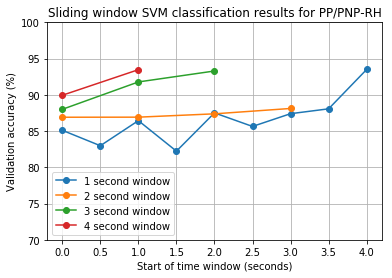
\includegraphics[scale=0.85]{rh.png}
\end{center}
\caption{\label{fig-slid-w-rh}Sliding window classification with band power + PCA and SVM on PP/PNP-RH}
\end{figure*}

\subsection{PCA weights per channel and power band}

In order to better understand how PCA extracts information from the various channels and power bands when reducing dimensionality, we plotted heat maps of the weights assigned by the PCA algorithm to each channel and power band. There are three plots for each data set (one plot per component), where warmer colours denote channels and power bands that had higher weights, and thus had a bigger impact on the final components that were used in classification.

Heat maps for PP/PNP-RH are displayed.

\begin{figure*}
\begin{center}
\hspace*{-2cm}
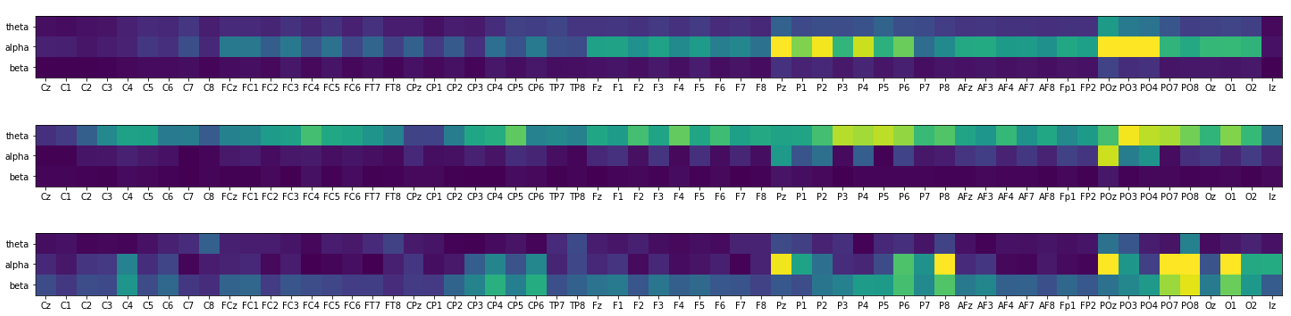
\includegraphics[scale=0.77]{pca_bp_rh_pp_pnp.PNG}
\end{center}
\caption{\label{fig-htmp-rh}Channels/power bands heat maps for three components, PP/PNP-RH}
\end{figure*}

\section{Discussion}

\subsection{Relevance of results}

\subsection{Future work}

try more classifiers

larger dataset

validation but no test

\section{Conclusions}


{\bf Acknowledgments.}
This is optional; it is a location for you to thank people

\bibliographystyle{abbrv}
\bibliography{references}


\end{document}